\documentclass[11pt,a4paper]{article}

\usepackage[a4paper,margin=1in]{geometry}
\usepackage[T1]{fontenc}
\usepackage[utf8]{inputenc}
\usepackage{newtxtext}
\usepackage{newtxmath}
\usepackage{microtype}
\usepackage{setspace}
\usepackage{graphicx}
\usepackage{float}
\usepackage{booktabs}
\usepackage{longtable}
\usepackage{tabularx}
\usepackage{array}
\usepackage{multirow}
\usepackage{xcolor}
\usepackage{hyperref}
\usepackage{enumitem}
\usepackage{amsmath}
\usepackage{listings}
\usepackage{caption}
\usepackage{subcaption}
\usepackage{tikz}
\usepackage{titlesec}
\usepackage{fancyhdr}
\usetikzlibrary{arrows.meta,positioning,fit,shapes.geometric}

\hypersetup{
  colorlinks=true,
  linkcolor=blue!60!black,
  urlcolor=blue!60!black,
  citecolor=blue!60!black
}

\setstretch{1.08}
\setlength{\parskip}{0.35em}
\setlength{\parindent}{0pt}

\definecolor{Accent}{HTML}{1F4E79}
\definecolor{SoftGray}{HTML}{F4F6F8}
\definecolor{DarkGray}{HTML}{404040}
\definecolor{CodeBg}{HTML}{F7F7F7}
\newcommand{\projecttitle}{Product Review Sentiment Analyzer for E-commerce}
\newcommand{\coursename}{DA5402 MLOps Final Project}

\titleformat{\section}{\Large\bfseries\color{Accent}}{\thesection}{0.75em}{}
\titleformat{\subsection}{\large\bfseries\color{DarkGray}}{\thesubsection}{0.75em}{}
\titleformat{\subsubsection}{\normalsize\bfseries\color{DarkGray}}{\thesubsubsection}{0.75em}{}
\titlespacing*{\section}{0pt}{1.1em}{0.5em}
\titlespacing*{\subsection}{0pt}{0.9em}{0.35em}
\captionsetup{font=small,labelfont=bf}

\pagestyle{fancy}
\fancyhf{}
\fancyhead[L]{\projecttitle}
\fancyhead[R]{\coursename}
\fancyfoot[C]{\thepage}
\renewcommand{\headrulewidth}{0.35pt}
\renewcommand{\footrulewidth}{0pt}

\lstset{
  basicstyle=\ttfamily\small,
  backgroundcolor=\color{CodeBg},
  frame=single,
  breaklines=true,
  columns=fullflexible
}

\newcommand{\evidencefigure}[3][0.92\linewidth]{
  \begin{figure}[H]
    \centering
    \IfFileExists{screenshots/#2}{
      \includegraphics[width=#1]{screenshots/#2}
    }{
      \fbox{
        \parbox[c][2.5in][c]{0.84\linewidth}{
          \centering
          Screenshot placeholder\\[0.5em]
          Upload the file\\
          \texttt{screenshots/#2}
        }
      }
    }
    \caption{#3}
  \end{figure}
}

\newcommand{\smallmetric}[2]{\textbf{#1}: #2}

\begin{document}

\begin{titlepage}
  \thispagestyle{empty}
  \centering
  \vspace*{2.4cm}
  {\Large \coursename \par}
  \vspace{1.6cm}
  {\LARGE \bfseries \projecttitle \par}
  \vspace{2.1cm}
  {\large Final Project Report \par}
  \vspace{1.8cm}
  {\large Submitted by \par}
  \vspace{0.4cm}
  {\Large Akshay Ambekar \par}
  \vspace{0.25cm}
  {\large Roll No.: DA25S007 \par}
  \vfill
  {\large April 2026 \par}
\end{titlepage}
\clearpage
\tableofcontents
\clearpage

\section{Executive Summary}

This report documents the complete design, implementation, automation, deployment, monitoring, and validation journey of an end-to-end AI application built for product review sentiment analysis in the e-commerce domain. The project was intentionally designed to maximize MLOps completeness rather than model novelty. The final system combines a React/Vite frontend, a FastAPI inference backend, DVC-based reproducible pipelines, MLflow-based experiment tracking and model packaging, Airflow-based operational orchestration, Prometheus and Grafana based observability, AlertManager-based alert routing, and Docker Compose based local deployment.

The final trained model uses a sparse classical NLP pipeline rather than a transformer. This choice was deliberate. The course constraints disallow cloud resources and emphasize reproducibility, automation, explainability, and local deployment. A TF-IDF based model family allowed the project to satisfy these constraints while still producing a useful application with explainable token-level reasoning and very small model artifacts.

The strongest outcomes from the current artifact snapshot are summarized below.

\begin{itemize}[leftmargin=1.4em]
  \item A balanced dataset of \textbf{15{,}000} English Amazon-style product reviews was ingested from \texttt{SetFit/amazon\_reviews\_multi\_en}, with \textbf{5{,}000} reviews in each class after the rating-to-sentiment mapping.
  \item Automated preprocessing removed \textbf{13 duplicate reviews}, leaving \textbf{14{,}987} usable rows and deterministic train/validation/test splits of \textbf{10{,}490 / 2{,}248 / 2{,}249}.
  \item The training pipeline compared \textbf{5 candidate models}. The selected model was \textbf{tfidf\_logistic\_tuned}.
  \item The selected model achieved \textbf{test accuracy = 0.7741}, \textbf{test macro F1 = 0.7737}, and \textbf{evaluation latency = 0.02895 ms/review} on the held-out test set, satisfying the configured acceptance gates of macro F1 $\ge 0.75$ and latency $< 200$ ms/review.
  \item The exported model artifact size is \textbf{5.02 MB}, and the model is packaged both as a local \texttt{joblib} artifact and an \texttt{MLflow pyfunc} serving artifact.
  \item The current DVC pipeline report shows a complete end-to-end lifecycle run in \textbf{24.14 seconds} on local hardware.
  \item Drift monitoring is active. The latest drift report shows a \textbf{drift score of 0.0926}, below the configured threshold of \textbf{0.25}.
  \item The maintenance policy examined \textbf{61 feedback records}, found \textbf{0 corrections}, and therefore decided to \textbf{continue monitoring} rather than trigger retraining.
  \item The automated test suite currently reports \textbf{41 passed, 1 skipped} on 24 April 2026.
\end{itemize}

\section{Problem Definition and Project Goals}

\subsection{Business Problem}

E-commerce platforms receive a high volume of product reviews every day. Manually reading and summarizing these reviews is slow, inconsistent, and difficult to scale. The goal of this project is to build a deployable AI application that accepts a user-provided product review and predicts whether the sentiment is \texttt{positive}, \texttt{neutral}, or \texttt{negative}. The system must also expose enough operational information to support real-world maintenance.

\subsection{Why This Problem Was Chosen}

The professor explicitly emphasized that the final project would be graded more heavily on \emph{MLOps quality} than on the creativity of the problem statement. Product review sentiment analysis is a good fit for that requirement because it naturally supports:

\begin{itemize}[leftmargin=1.4em]
  \item deterministic data ingestion and preprocessing,
  \item multiple model experiments,
  \item explainable inference,
  \item API-based deployment,
  \item feedback collection,
  \item drift detection,
  \item retraining policy automation,
  \item monitoring dashboards and alerts.
\end{itemize}

\subsection{Project Objectives}

The project was designed to satisfy both ML objectives and business/operations objectives.

\begin{table}[H]
  \centering
  \caption{Configured project objectives}
  \begin{tabularx}{\linewidth}{>{\raggedright\arraybackslash}p{0.27\linewidth}X}
    \toprule
    \textbf{Objective Type} & \textbf{Target} \\
    \midrule
    Business objective & Interactive review sentiment prediction through a non-technical frontend \\
    Business objective & Deployment as separate frontend and backend services over REST \\
    Business objective & Health and readiness visibility through dedicated endpoints \\
    Business objective & Monitoring for availability, latency, errors, data drift, and retraining conditions \\
    ML objective & Macro F1 $\ge 0.75$ on held-out test data \\
    ML objective & Explainable token-level reasoning for predictions \\
    MLOps objective & Full lifecycle reproducibility through Git, DVC, MLflow, and containerized execution \\
    MLOps objective & Automated operational workflows through Airflow, Prometheus, Grafana, AlertManager, and GitHub Actions \\
    \bottomrule
  \end{tabularx}
\end{table}

\section{Why This Toolchain Was Chosen}

The tool choices were not accidental; they were selected to align with the course rubric.

\begin{table}[H]
  \centering
  \caption{Core tools and why they are present in the system}
  \begin{tabularx}{\linewidth}{>{\raggedright\arraybackslash}p{0.18\linewidth}>{\raggedright\arraybackslash}p{0.24\linewidth}X}
    \toprule
    \textbf{Tool} & \textbf{Role in Project} & \textbf{Why it matters here} \\
    \midrule
    Git & Source control & Tracks code evolution, release history, and traceability of every experiment \\
    DVC & Data/model pipeline versioning & Encodes lifecycle stages, parameters, artifacts, metrics, plots, and reproducibility \\
    MLflow & Experiment tracking + model packaging & Records runs, parameters, metrics, artifacts, and model registry entries \\
    Airflow & Operational orchestration & Provides a visible pipeline console, scheduling, retries, dynamic workflow behavior, and retraining triggers \\
    FastAPI & Inference and operations API & Exposes prediction, health, readiness, feedback, metrics, and operational endpoints \\
    React/Vite & Frontend UI & Provides a responsive, non-technical user experience and keeps frontend/backend loosely coupled \\
    Docker Compose & Deployment & Enforces environment parity and packages the full stack locally \\
    Prometheus & Metrics collection & Scrapes application and infrastructure telemetry \\
    Grafana & Visualization & Displays health, throughput, latency, drift, and pipeline state in near real time \\
    AlertManager & Alert routing & Handles alert grouping, inhibition, and notification delivery \\
    Node Exporter & System monitoring & Adds host CPU, memory, and disk signals for infrastructure correlation \\
    GitHub Actions & CI/CD & Automates linting, testing, DVC reproduction, Docker validation, and deployment smoke tests \\
    \bottomrule
  \end{tabularx}
\end{table}

\section{System Overview}

\subsection{High-Level Architecture}

The system follows a loosely coupled multi-service architecture. The frontend and backend communicate only through REST. Training and orchestration are separate from inference. Monitoring is externalized through Prometheus, Grafana, and AlertManager. This separation was important both architecturally and for scoring under the deployment and design-principles criteria.

\begin{figure}[H]
  \centering
  \resizebox{0.96\linewidth}{!}{
  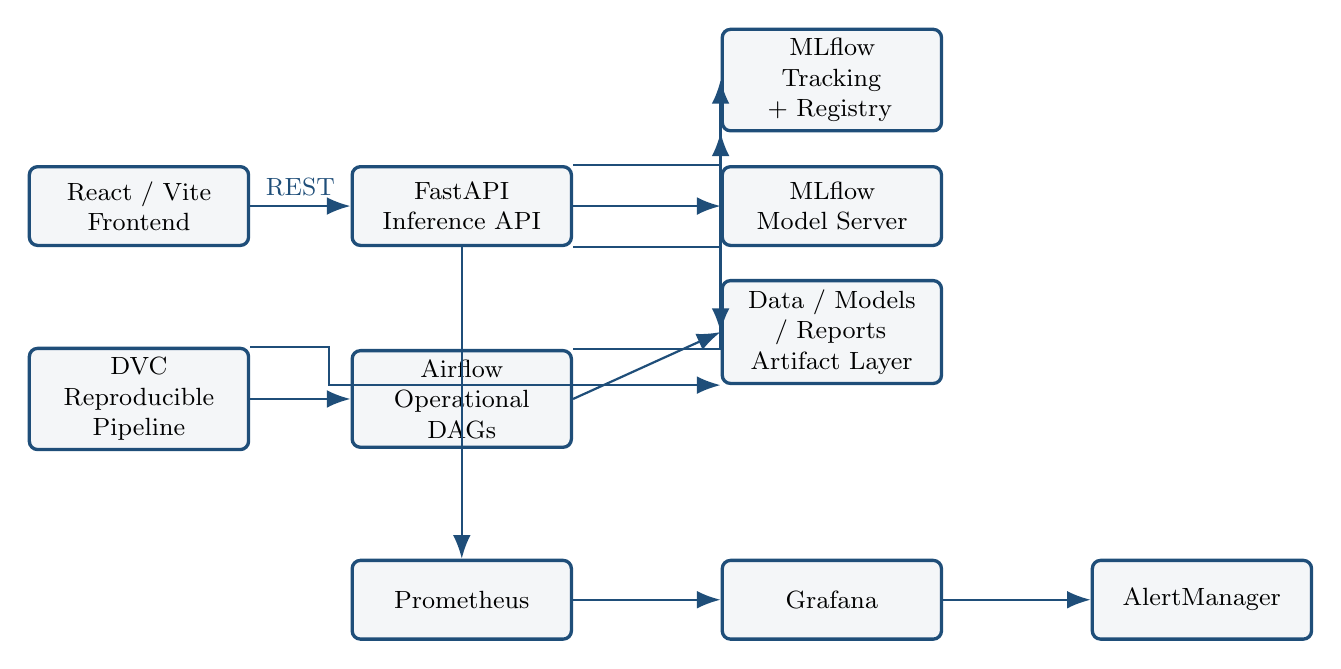
\begin{tikzpicture}[
    font=\small,
    box/.style={draw=Accent, rounded corners=3pt, very thick, fill=SoftGray, align=center, text width=2.55cm, minimum height=1.0cm},
    arrow/.style={-{Latex[length=3mm]}, thick, Accent}
  ]
    \node[box] (frontend) at (0,0) {React / Vite\\Frontend};
    \node[box] (api) at (4.1,0) {FastAPI\\Inference API};
    \node[box] (mlflow) at (8.8,1.6) {MLflow\\Tracking + Registry};
    \node[box] (modelserver) at (8.8,0.0) {MLflow\\Model Server};
    \node[box] (artifacts) at (8.8,-1.6) {Data / Models / Reports\\Artifact Layer};
    \node[box] (dvc) at (0,-2.45) {DVC\\Reproducible Pipeline};
    \node[box] (airflow) at (4.1,-2.45) {Airflow\\Operational DAGs};
    \node[box] (prom) at (4.1,-5.0) {Prometheus};
    \node[box] (grafana) at (8.8,-5.0) {Grafana};
    \node[box] (alertmanager) at (13.5,-5.0) {AlertManager};

    \draw[arrow] (frontend) -- node[above] {REST} (api);
    \draw[arrow] (api.east) -- (modelserver.west);
    \draw[arrow] (api.north east) -| (mlflow.west);
    \draw[arrow] (api.south east) -| (artifacts.west);
    \draw[arrow] (dvc.east) -- (airflow.west);
    \draw[arrow] (dvc.north east) -- ++(1.0,0) |- (artifacts.south west);
    \draw[arrow] (airflow.east) -- (artifacts.west);
    \draw[arrow] (airflow.north east) -| (mlflow.south west);
    \draw[arrow] (api.south) -- (prom.north);
    \draw[arrow] (prom.east) -- (grafana.west);
    \draw[arrow] (grafana.east) -- (alertmanager.west);
  \end{tikzpicture}
  }
  \caption{High-level architecture of the local MLOps system}
\end{figure}

\subsection{Docker Compose Services}

The deployed local stack consists of these long-running services:

\begin{itemize}[leftmargin=1.4em]
  \item \texttt{frontend}
  \item \texttt{api}
  \item \texttt{mlflow}
  \item \texttt{mlflow-model-server}
  \item \texttt{postgres}
  \item \texttt{airflow-webserver}
  \item \texttt{airflow-scheduler}
  \item \texttt{airflow-dag-processor}
  \item \texttt{prometheus}
  \item \texttt{grafana}
  \item \texttt{alertmanager}
  \item \texttt{node-exporter}
\end{itemize}

At the time of report preparation, all health-critical services in the local stack were up and healthy.

\subsection{Frontend / Backend Loose Coupling}

The frontend does not import backend modules or model code directly. It only calls the backend through configurable REST endpoints. The backend does not know about frontend implementation details. This clean split was a deliberate design requirement from the rubric.

\section{End-to-End ML Lifecycle}

\begin{figure}[H]
  \centering
  \resizebox{\linewidth}{!}{
  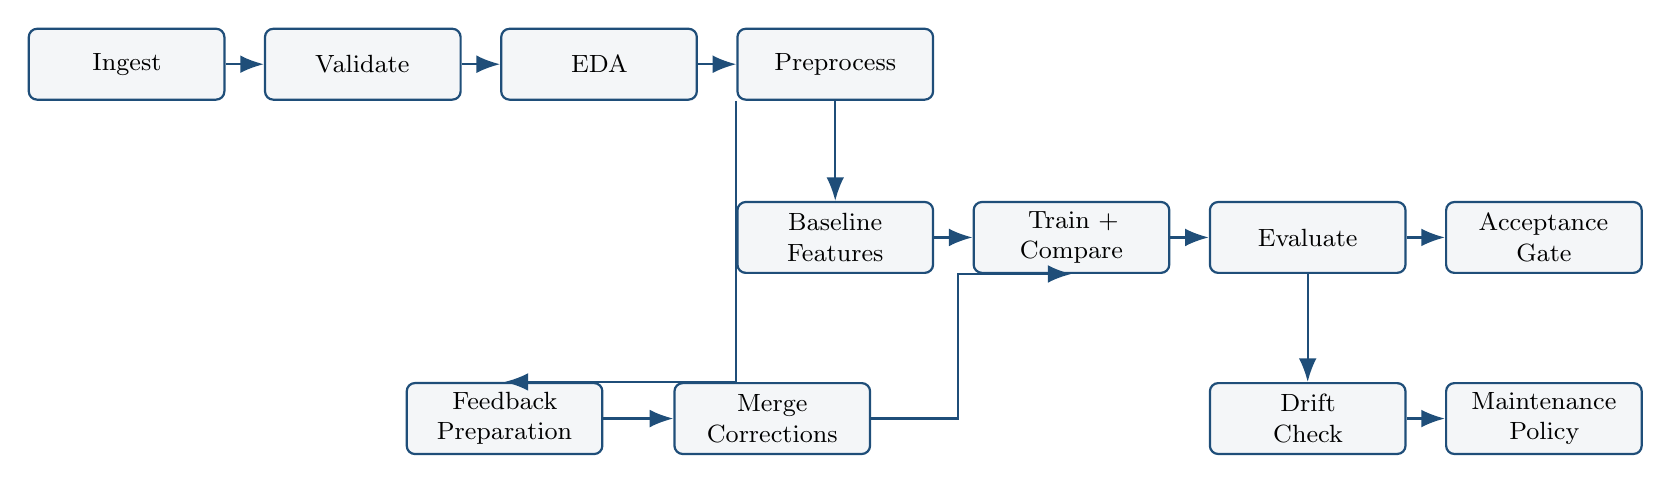
\begin{tikzpicture}[
    font=\small,
    stage/.style={draw=Accent, rounded corners=3pt, thick, fill=SoftGray, text width=2.25cm, minimum height=0.9cm, align=center},
    arrow/.style={-{Latex[length=3mm]}, thick, Accent}
  ]
    \node[stage] (ingest) at (0,0) {Ingest};
    \node[stage] (validate) at (3.0,0) {Validate};
    \node[stage] (eda) at (6.0,0) {EDA};
    \node[stage] (prep) at (9.0,0) {Preprocess};
    \node[stage] (feature) at (9.0,-2.2) {Baseline\\Features};
    \node[stage] (train) at (12.0,-2.2) {Train +\\Compare};
    \node[stage] (eval) at (15.0,-2.2) {Evaluate};
    \node[stage] (accept) at (18.0,-2.2) {Acceptance\\Gate};
    \node[stage] (feedback) at (4.8,-4.5) {Feedback\\Preparation};
    \node[stage] (merge) at (8.2,-4.5) {Merge\\Corrections};
    \node[stage] (drift) at (15.0,-4.5) {Drift\\Check};
    \node[stage] (maint) at (18.0,-4.5) {Maintenance\\Policy};

    \draw[arrow] (ingest) -- (validate);
    \draw[arrow] (validate) -- (eda);
    \draw[arrow] (eda) -- (prep);
    \draw[arrow] (prep) -- (feature);
    \draw[arrow] (feature) -- (train);
    \draw[arrow] (train) -- (eval);
    \draw[arrow] (eval) -- (accept);
    \draw[arrow] (prep.south west) |- (feedback.north);
    \draw[arrow] (feedback) -- (merge);
    \draw[arrow] (merge.east) -- ++(1.1,0) |- (train.south);
    \draw[arrow] (eval.south) -- (drift.north);
    \draw[arrow] (drift) -- (maint);
  \end{tikzpicture}
  }
  \caption{Logical lifecycle implemented by DVC, Airflow, and the supporting Python modules}
\end{figure}

\section{Data Collection and Data Understanding}

\subsection{Dataset Choice}

The project uses the public dataset \texttt{SetFit/amazon\_reviews\_multi\_en}. This choice provided real product review text, rating labels, and enough volume for meaningful experimentation while remaining lightweight enough for local-only execution.

The pipeline ingests the data into a normalized schema:

\begin{lstlisting}
review_id: string
review_text: string
rating: integer
sentiment: string
source: string
ingested_at: datetime
\end{lstlisting}

Sentiment labels are derived from ratings as follows:

\begin{itemize}[leftmargin=1.4em]
  \item ratings 1--2 $\rightarrow$ \texttt{negative}
  \item rating 3 $\rightarrow$ \texttt{neutral}
  \item ratings 4--5 $\rightarrow$ \texttt{positive}
\end{itemize}

\subsection{Automated Ingestion}

The ingestion stage is automated in code and encoded in both DVC and Airflow. The latest artifact snapshot shows:

\begin{itemize}[leftmargin=1.4em]
  \item \smallmetric{Source rows seen}{165{,}000}
  \item \smallmetric{Rows kept for project}{15{,}000}
  \item \smallmetric{Dataset used}{\texttt{SetFit/amazon\_reviews\_multi\_en}}
  \item \smallmetric{Fallback mode used}{No}
\end{itemize}

The project deliberately caps the ingested dataset to a fixed size in order to keep the local training loop fast and reproducible.

\subsection{Automated Data Validation}

Data validation is performed immediately after ingestion. The validator checks:

\begin{itemize}[leftmargin=1.4em]
  \item schema completeness,
  \item null values,
  \item duplicate review IDs,
  \item duplicate review text,
  \item invalid ratings,
  \item invalid sentiment labels,
  \item empty reviews,
  \item class presence,
  \item class imbalance.
\end{itemize}

The latest validation report found no blocking errors, but it did surface two warnings:

\begin{itemize}[leftmargin=1.4em]
  \item \textbf{13 duplicate review texts}
  \item \textbf{1 mixed-label duplicate text}
\end{itemize}

This is useful because the pipeline does not silently assume perfect data. It records quality observations as part of the lifecycle evidence.

\subsection{EDA Results}

Exploratory data analysis is automated rather than done only in a notebook. The current EDA artifact snapshot shows:

\begin{itemize}[leftmargin=1.4em]
  \item \smallmetric{Rows analyzed}{15{,}000}
  \item \smallmetric{Mean review length}{169.10 characters}
  \item \smallmetric{Median review length}{118 characters}
  \item \smallmetric{95th percentile review length}{472.05 characters}
  \item \smallmetric{99th percentile review length}{828.01 characters}
  \item \smallmetric{Missing values}{0 in all required fields}
  \item \smallmetric{Class distribution}{5{,}000 negative, 5{,}000 neutral, 5{,}000 positive}
\end{itemize}

The EDA stage also produces figures for:

\begin{itemize}[leftmargin=1.4em]
  \item class distribution,
  \item rating distribution,
  \item text length distribution,
  \item top-token volume by sentiment.
\end{itemize}

\evidencefigure{eda_class_distribution.png}{Screenshot placeholder for the class-distribution or EDA visual generated from the report artifacts}
\evidencefigure{eda_text_length_distribution.png}{Screenshot placeholder for the text-length distribution figure}

\subsection{Bias and Limitation Awareness}

The project explicitly documents several data limitations:

\begin{itemize}[leftmargin=1.4em]
  \item The dataset is English-only.
  \item Sentiment labels are derived from ratings rather than direct human sentiment annotation.
  \item A rating of 3 is treated as neutral, even though some 3-star reviews contain mixed language.
  \item Product category metadata is limited in the reduced schema used here.
\end{itemize}

This matters because good MLOps practice includes documenting where the data may systematically misrepresent real-world behavior.

\section{Preprocessing and Feature Engineering}

\subsection{Why Preprocessing Exists as a Separate Stage}

Feature engineering logic should not be mixed casually into model training. This project keeps preprocessing and feature baseline creation as explicit, versioned lifecycle steps. That separation makes the pipeline easier to reproduce, debug, and explain.

\subsection{Cleaning Logic}

The preprocessing stage:

\begin{itemize}[leftmargin=1.4em]
  \item normalizes whitespace,
  \item rejects empty reviews,
  \item rejects reviews below the minimum text length,
  \item rejects reviews above the maximum text length,
  \item removes duplicate normalized review text,
  \item writes rejected rows to a separate audit file.
\end{itemize}

This is important from an MLOps perspective because rejected rows are not silently discarded. They are preserved in an auditable artifact.

\subsection{Current Preprocessing Outcome}

The latest preprocessing report shows:

\begin{itemize}[leftmargin=1.4em]
  \item \smallmetric{Input rows}{15{,}000}
  \item \smallmetric{Rejected rows}{13}
  \item \smallmetric{Final rows}{14{,}987}
  \item \smallmetric{Rows removed due to duplicates}{13}
  \item \smallmetric{Rows removed due to empty text}{0}
  \item \smallmetric{Rows removed due to short text}{0}
  \item \smallmetric{Rows removed due to long text}{0}
\end{itemize}

\subsection{Deterministic Splits}

The split is deterministic and driven by a fixed seed in \texttt{params.yaml}. The resulting split sizes are:

\begin{table}[H]
  \centering
  \caption{Current processed dataset split}
  \begin{tabular}{lrrr}
    \toprule
    \textbf{Split} & \textbf{Rows} & \textbf{Negative} & \textbf{Neutral / Positive} \\
    \midrule
    Train & 10{,}490 & 3{,}496 & 3{,}498 / 3{,}496 \\
    Validation & 2{,}248 & 750 & 749 / 749 \\
    Test & 2{,}249 & 749 & 750 / 750 \\
    \bottomrule
  \end{tabular}
\end{table}

This balance matters because model comparison becomes much easier to interpret when all three classes remain well represented in every split.

\subsection{Feature Baseline for Drift Monitoring}

The feature-engineering stage computes and stores baseline statistics used later for drift detection. The current baseline report confirms that:

\begin{itemize}[leftmargin=1.4em]
  \item \textbf{50 tracked TF-IDF feature means} were stored
  \item \textbf{50 tracked TF-IDF feature variances} were stored
\end{itemize}

This satisfies the requirement to capture baseline feature statistics during the data-engineering phase so that future distributions can be compared against training-time behavior.

\section{Model Development, Experiment Tracking, and Selection}

\subsection{Why a Classical Model Was Chosen}

The final model family uses sparse bag-of-words style representations rather than a transformer. This decision was based on the project constraints:

\begin{itemize}[leftmargin=1.4em]
  \item The course forbids cloud usage.
  \item The system must be easy to retrain locally.
  \item The deployment must be fast and lightweight.
  \item The model should remain explainable for the demo.
\end{itemize}

A linear text classifier satisfies these conditions much better than a transformer for this specific assignment.

\subsection{Candidate Models}

The project compares five candidates, all defined in \texttt{params.yaml}. This allows model experimentation to remain parameter-driven rather than hardcoded.

\begin{table}[H]
  \centering
  \caption{Candidate models and observed results from the latest training run}
  \small
  \begin{tabularx}{\linewidth}{>{\raggedright\arraybackslash}X>{\centering\arraybackslash}p{0.12\linewidth}>{\centering\arraybackslash}p{0.12\linewidth}>{\centering\arraybackslash}p{0.18\linewidth}>{\centering\arraybackslash}p{0.11\linewidth}}
    \toprule
    \textbf{Candidate} & \textbf{Val. F1} & \textbf{Test F1} & \textbf{Latency (ms/review)} & \textbf{Accepted} \\
    \midrule
    TF-IDF + Logistic (baseline) & 0.7650 & 0.7593 & 0.0313 & Yes \\
    TF-IDF + Logistic (regularized) & 0.7746 & 0.7720 & 0.0248 & Yes \\
    TF-IDF + Logistic (tuned) & 0.7750 & 0.7737 & 0.0399 & Yes \\
    TF-IDF + SGD log-loss & 0.7679 & 0.7686 & 0.0351 & Yes \\
    Count + Multinomial NB & 0.7743 & 0.7747 & 0.0284 & Yes \\
    \bottomrule
  \end{tabularx}
\end{table}

\subsection{Selection Rule}

The model-selection rule is intentionally explicit:

\begin{quote}
Choose the candidate with highest validation macro F1 among models that satisfy the test macro F1 and latency gates. If no candidate passes, choose the best validation macro F1 candidate and mark acceptance as failed.
\end{quote}

This rule matters because model promotion is not manual. The system does not simply choose a model by visual inspection after training; it uses a coded and reproducible selection policy.

\subsection{Selected Model and Final Offline Evaluation}

The selected model from the latest artifact snapshot is:

\begin{itemize}[leftmargin=1.4em]
  \item \smallmetric{Selected model}{\texttt{tfidf\_logistic\_tuned}}
  \item \smallmetric{Test accuracy}{0.7741}
  \item \smallmetric{Test macro precision}{0.7733}
  \item \smallmetric{Test macro recall}{0.7741}
  \item \smallmetric{Test macro F1}{0.7737}
  \item \smallmetric{Held-out evaluation latency}{0.02895 ms/review}
  \item \smallmetric{Acceptance gate}{Passed}
  \item \smallmetric{Model size}{5.02 MB}
\end{itemize}

\subsection{Confusion Matrix}

The selected model's confusion matrix on the held-out test split is:

\begin{table}[H]
  \centering
  \caption{Confusion matrix of the selected model on the held-out test set}
  \begin{tabular}{lccc}
    \toprule
    \textbf{Actual $\backslash$ Predicted} & \textbf{Negative} & \textbf{Neutral} & \textbf{Positive} \\
    \midrule
    Negative & 572 & 152 & 25 \\
    Neutral & 145 & 517 & 88 \\
    Positive & 24 & 74 & 652 \\
    \bottomrule
  \end{tabular}
\end{table}

The strongest class is \texttt{positive}, while \texttt{neutral} remains the hardest class. This is not unusual in rating-derived sentiment tasks, because neutral language often overlaps semantically with mild positive or mild negative review text.

\subsection{Explainability}

The model exports token-level feature importance for explainability. Since the chosen classifier is linear over sparse text features, class-specific token weights can be recovered and used in the UI. This was preferred over a black-box model because it makes the prediction easier to explain during the demo and viva.

\section{Reproducibility and Versioning}

\subsection{Why Reproducibility Is a Core Requirement}

The central MLOps promise is not only that a model can be trained once, but that it can be trained again under controlled conditions and traced back to specific code, data, and configuration states. This project therefore records reproducibility information in multiple layers.

\subsection{Git}

Git tracks source code evolution, release tags, and repository history. In this project, Git is the source-of-truth layer for application code, pipeline definitions, infrastructure configuration, and report files, while DVC and MLflow provide the data and experiment layers built on top of that codebase.

\subsection{DVC}

DVC is used to:

\begin{itemize}[leftmargin=1.4em]
  \item define staged lifecycle steps in \texttt{dvc.yaml},
  \item track parameterized stage dependencies,
  \item version raw data, processed data, and model artifacts,
  \item record metrics and plots,
  \item reproduce the pipeline with \texttt{dvc repro},
  \item maintain a lock file that records the exact executed state.
\end{itemize}

The lifecycle stages include:

\begin{lstlisting}
ingest -> validate -> eda -> preprocess -> prepare_feedback
      -> merge_feedback -> featurize -> train -> evaluate
      -> accept -> drift -> publish
\end{lstlisting}

\evidencefigure{dvc_dag.png}{Screenshot placeholder for the DVC DAG or DVC stage graph}

\subsection{MLflow}

MLflow is used for:

\begin{itemize}[leftmargin=1.4em]
  \item experiment tracking,
  \item metric logging,
  \item parameter logging,
  \item artifact logging,
  \item model registration,
  \item pyfunc model packaging.
\end{itemize}

Every candidate model gets its own MLflow run. This means the training loop is traceable not only at the final-model level but also at the experiment-comparison level.

\subsection{Combined Traceability}

The project therefore supports this traceability chain:

\begin{quote}
Git versioned source $\rightarrow$ DVC pipeline state $\rightarrow$ MLflow run ID $\rightarrow$ model artifact $\rightarrow$ deployed API response.
\end{quote}

\section{Workflow Orchestration: DVC and Airflow}

\subsection{Why Both DVC and Airflow Are Present}

At first glance, DVC and Airflow seem to overlap. In fact, they serve different purposes:

\begin{itemize}[leftmargin=1.4em]
  \item \textbf{DVC} encodes reproducibility, parameter dependency tracking, data/model versioning, and offline re-execution.
  \item \textbf{Airflow} provides scheduling, retries, task logs, run history, dynamic workflow behavior, and a visible pipeline console.
\end{itemize}

The two systems intentionally orchestrate the same lifecycle modules at different layers. This is not redundant business logic; it is a reproducibility view plus an operations view of the same pipeline.

\subsection{Training DAG}

The Airflow training DAG orchestrates the end-to-end training lifecycle. The tasks cover:

\begin{itemize}[leftmargin=1.4em]
  \item data ingestion,
  \item raw data validation,
  \item EDA,
  \item preprocessing,
  \item feature baseline generation,
  \item model training and comparison,
  \item evaluation,
  \item acceptance gating,
  \item drift checking,
  \item pipeline report publication.
\end{itemize}

\subsection{Batch Ingestion DAG}

The project also includes a separate Airflow batch ingestion DAG for operational data engineering behavior. This DAG can process incoming files, chunk them, quarantine malformed data, and produce operational reports. The current batch pipeline evidence includes a negative scenario:

\begin{itemize}[leftmargin=1.4em]
  \item \smallmetric{Source file}{\texttt{demo\_bad\_batch\_alert.csv}}
  \item \smallmetric{Failure reason}{Missing required column \texttt{review\_text}}
  \item \smallmetric{Action taken}{File quarantined}
\end{itemize}

This negative-path behavior matters because it demonstrates fault-aware orchestration rather than a happy-path-only pipeline.

\evidencefigure{airflow_training_runs.png}{Screenshot placeholder for the Airflow training DAG run history}
\evidencefigure{airflow_batch_quarantine.png}{Screenshot placeholder for the Airflow batch-ingestion failure/quarantine scenario}

\subsection{Pipeline Throughput Evidence}

The current pipeline performance report provides per-stage timing and throughput. Selected examples are shown below.

\begin{table}[H]
  \centering
  \caption{Selected throughput and timing figures from the latest pipeline performance report}
  \begin{tabularx}{\linewidth}{>{\raggedright\arraybackslash}p{0.33\linewidth}rrX}
    \toprule
    \textbf{Stage} & \textbf{Duration (s)} & \textbf{Rows} & \textbf{Throughput (rows/s)} \\
    \midrule
    Ingest data & 12.81 & 165{,}000 source rows seen & 12{,}879.92 \\
    Validate raw data & 0.105 & 15{,}000 & 142{,}799.97 \\
    Run EDA & 1.398 & 15{,}000 & 10{,}730.19 \\
    Preprocess data & 0.147 & 15{,}000 & 101{,}825.10 \\
    Compute drift baseline & 0.542 & 10{,}490 & 19{,}354.18 \\
    Train and compare models & 8.562 & 14{,}987 combined rows & 1{,}750.38 \\
    Evaluate selected model & 0.323 & 2{,}249 & 6{,}963.99 \\
    Batch drift check & 0.030 & 2{,}249 & 74{,}786.66 \\
    \bottomrule
  \end{tabularx}
\end{table}

The total duration of the latest complete pipeline run is \textbf{24.14 seconds}.

\section{Model Serving and Application API}

\subsection{Serving Strategy}

The project uses a hybrid serving approach:

\begin{itemize}[leftmargin=1.4em]
  \item \textbf{FastAPI} provides the main interactive application API.
  \item \textbf{MLflow pyfunc packaging} provides a separate model-serving artifact and a separate MLflow model server service.
\end{itemize}

This means the system is not tied to a single in-process inference path. The model is available both as a local \texttt{joblib} artifact for the application and as an MLflow-packaged model.

\subsection{Model Artifacts}

The training stage exports:

\begin{itemize}[leftmargin=1.4em]
  \item \texttt{models/sentiment\_model.joblib}
  \item \texttt{models/model\_metadata.json}
  \item \texttt{models/feature\_importance.json}
  \item \texttt{models/mlflow\_model/}
\end{itemize}

\subsection{Application Endpoints}

\begin{table}[H]
  \centering
  \caption{Primary FastAPI endpoints}
  \small
  \begin{tabularx}{\linewidth}{>{\raggedright\arraybackslash\ttfamily}p{0.27\linewidth}>{\raggedright\arraybackslash}p{0.11\linewidth}>{\raggedright\arraybackslash}X}
    \toprule
    \textbf{Endpoint} & \textbf{Method} & \textbf{Purpose} \\
    \midrule
    /health & GET & Process-level health check \\
    /ready & GET & Readiness check based on model loading \\
    /predict & POST & Interactive inference for a review \\
    /feedback & POST & Ground-truth feedback submission \\
    /model/info & GET & Model metadata and serving mode \\
    \shortstack[l]{/metrics-\\summary} & GET & Human-oriented summary of lifecycle and monitoring state \\
    /metrics & GET & Prometheus metrics exposition endpoint \\
    \shortstack[l]{/monitoring/\\refresh} & POST & Forces report-metric refresh \\
    /ops/alerts & POST & Demo alert receiver endpoint \\
    \bottomrule
  \end{tabularx}
\end{table}

\subsection{Interactive Prediction Behavior}

At inference time, the API:

\begin{enumerate}[leftmargin=1.6em]
  \item validates the incoming request,
  \item loads the trained sklearn pipeline,
  \item predicts sentiment,
  \item computes class probabilities,
  \item derives explanation tokens from saved feature importance,
  \item measures latency,
  \item returns model version and MLflow run information,
  \item updates Prometheus metrics.
\end{enumerate}

The frontend therefore receives not just a label, but a full inference payload with supporting evidence.

\evidencefigure{frontend_prediction.png}{Screenshot placeholder for the main prediction UI}
\evidencefigure{frontend_mlops_dashboard.png}{Screenshot placeholder for the frontend MLOps dashboard}

\section{Monitoring, Alerting, and Maintenance}

\subsection{Prometheus-Based Instrumentation}

The API exports detailed Prometheus metrics. The monitored information includes:

\begin{itemize}[leftmargin=1.4em]
  \item request count by endpoint, method, and status code,
  \item request latency histogram,
  \item active request gauge,
  \item error count,
  \item invalid-review rejection count,
  \item prediction count by sentiment,
  \item model inference latency histogram,
  \item review text length summary,
  \item process memory usage,
  \item process CPU usage,
  \item model loaded / fallback mode / acceptance state,
  \item drift score and drift-detected flag,
  \item pipeline duration and per-stage throughput,
  \item batch rows processed, failed chunks, and quarantine status,
  \item feedback counters, feedback accuracy ratio, observed feedback count, correction count, and recent corrections,
  \item maintenance policy outputs such as retraining-required state and active retraining reasons.
\end{itemize}

This is more than basic health monitoring; it provides observability across the API, model, data, and lifecycle layers.

\subsection{Grafana Dashboards}

Grafana now exposes two intentionally different dashboards rather than one overloaded screen:

\begin{itemize}[leftmargin=1.4em]
  \item \textbf{Sentiment System Overview}: a broad MLOps summary for the complete project state
  \item \textbf{Sentiment Operations and SLOs}: a more operational view for live service behavior, SLOs, and alert triage
\end{itemize}

The \textbf{Sentiment System Overview} dashboard summarizes:

\begin{itemize}[leftmargin=1.4em]
  \item API availability,
  \item model loaded / fallback / acceptance state,
  \item retraining decision,
  \item drift score,
  \item test macro F1,
  \item rejected-row ratio,
  \item feedback accuracy and recent corrections,
  \item pipeline duration and pipeline-stage timing,
  \item batch pipeline outcomes,
  \item infrastructure health and alert counts.
\end{itemize}

The \textbf{Sentiment Operations and SLOs} dashboard focuses on:

\begin{itemize}[leftmargin=1.4em]
  \item request rate and request outcome by status code,
  \item p95 inference latency and request latency by endpoint,
  \item prediction distribution rate,
  \item active requests,
  \item invalid-review rate by reason,
  \item API versus host CPU correlation,
  \item API process memory,
  \item model/drift state,
  \item retraining signals,
  \item current firing alerts and alert-notification traffic.
\end{itemize}

\evidencefigure{grafana_system_overview.png}{Screenshot placeholder for the Grafana \texttt{Sentiment System Overview} dashboard}
\evidencefigure{grafana_operations_slos.png}{Screenshot placeholder for the Grafana \texttt{Sentiment Operations and SLOs} dashboard}

\subsection{Alert Rules}

The alert configuration covers multiple failure classes:

\begin{itemize}[leftmargin=1.4em]
  \item API unavailable,
  \item error rate above 5\%,
  \item invalid-review rate elevated,
  \item active request count too high,
  \item model not loaded,
  \item fallback mode active,
  \item model acceptance failed,
  \item data drift detected,
  \item pipeline duration too high,
  \item rejected-row ratio too high,
  \item batch file quarantined,
  \item batch chunk failures,
  \item p95 inference latency above 200 ms,
  \item infrastructure CPU, memory, and disk pressure,
  \item AlertManager and node exporter availability.
\end{itemize}

Two rubric-critical alert conditions are directly encoded:

\begin{itemize}[leftmargin=1.4em]
  \item \textbf{Error rate alert:} fires when recent API 5xx rate exceeds 5\%
  \item \textbf{Drift alert:} fires when the drift score exceeds 0.25 or the drift flag is set
\end{itemize}

\evidencefigure{prometheus_alerts.png}{Screenshot placeholder for Prometheus active alerts or alert rule view}
\evidencefigure{alertmanager_ui.png}{Screenshot placeholder for AlertManager grouping or received alerts}

\subsection{Drift Detection}

The drift detector compares the current data distribution against the training-time baseline using:

\begin{itemize}[leftmargin=1.4em]
  \item text-length mean movement,
  \item sentiment-distribution delta,
  \item TF-IDF feature-mean delta,
  \item TF-IDF feature-variance delta.
\end{itemize}

The final drift score is the maximum of these movement signals. The current drift evidence is:

\begin{itemize}[leftmargin=1.4em]
  \item \smallmetric{Drift threshold}{0.25}
  \item \smallmetric{Latest drift score}{0.0926}
  \item \smallmetric{Drift detected}{No}
  \item \smallmetric{Length delta ratio}{0.0386}
  \item \smallmetric{Sentiment distribution delta}{0.00023}
  \item \smallmetric{TF-IDF mean delta}{0.0926}
\end{itemize}

This indicates that the current observed data has not drifted enough to justify retraining.

\subsection{Feedback Loop}

The application collects user feedback through the \texttt{/feedback} endpoint. The maintenance logic currently sees:

\begin{itemize}[leftmargin=1.4em]
  \item \smallmetric{Feedback count}{61}
  \item \smallmetric{Matches}{61}
  \item \smallmetric{Corrections}{0}
  \item \smallmetric{Feedback accuracy}{1.0}
\end{itemize}

Only correction examples are converted into retraining-ready rows. This prevents the system from polluting the training set with duplicate confirmations that do not add new learning signal.

\subsection{Maintenance Policy and Retraining Logic}

The maintenance policy triggers retraining when any of the following conditions is true:

\begin{itemize}[leftmargin=1.4em]
  \item drift score exceeds the configured threshold,
  \item enough feedback has been collected and feedback accuracy drops below the threshold,
  \item enough recent corrections have been submitted within the correction window.
\end{itemize}

The current policy thresholds are:

\begin{itemize}[leftmargin=1.4em]
  \item drift threshold = 0.25
  \item minimum feedback count = 10
  \item minimum feedback accuracy = 0.8
  \item minimum recent corrections = 10
  \item correction window = 72 hours
  \item cooldown = 6 hours
\end{itemize}

The latest maintenance report concludes:

\begin{itemize}[leftmargin=1.4em]
  \item \smallmetric{Action}{\texttt{continue\_monitoring}}
  \item \smallmetric{Should retrain}{No}
  \item \smallmetric{Reasons}{None}
\end{itemize}

This is exactly what should happen in a healthy system: monitoring is active, policy evaluation is active, but unnecessary retraining is not triggered.

\section{Deployment, Packaging, and CI/CD}

\subsection{Container Strategy}

The system is packaged into separate containers for:

\begin{itemize}[leftmargin=1.4em]
  \item the frontend,
  \item the FastAPI backend,
  \item MLflow tracking,
  \item MLflow model serving,
  \item Airflow services,
  \item PostgreSQL,
  \item Prometheus,
  \item Grafana,
  \item AlertManager,
  \item node exporter.
\end{itemize}

This satisfies the rubric requirement that the frontend and backend remain independent software blocks connected only by configurable APIs.

\subsection{MLflow Packaging}

The training pipeline exports an MLflow pyfunc model under \texttt{models/mlflow\_model/}. That artifact can be served independently through the \texttt{mlflow-model-server} container.

\subsection{GitHub Actions CI/CD}

The CI/CD implementation contains four main jobs:

\begin{enumerate}[leftmargin=1.6em]
  \item \textbf{python}: installs dependencies, runs linting, runs tests, executes \texttt{dvc repro}, checks DVC status, uploads deployment artifacts
  \item \textbf{frontend}: installs frontend dependencies and builds the React app
  \item \textbf{configuration}: validates Docker Compose configuration and monitoring configuration
  \item \textbf{docker-deployment}: restores artifacts, builds deployment images, starts the local stack, runs smoke tests, and tears the stack down
\end{enumerate}

This is important because the deployment pipeline is not only documented; it is automated and tested.

\evidencefigure{github_actions_pipeline.png}{Screenshot placeholder for the GitHub Actions pipeline view}

\subsection{Rollback}

Rollback is supported through the model metadata and the rollback script. Since MLflow keeps multiple registered model versions, the serving layer can be redirected to a previous model version or stage by changing the deployment configuration and restarting the API service. This gives the project a credible operational recovery path when a newly promoted model is undesirable.

\section{Testing and Quality Assurance}

\subsection{Testing Strategy}

The test suite includes:

\begin{itemize}[leftmargin=1.4em]
  \item unit tests for data validation, EDA, preprocessing, model selection, acceptance gating, maintenance policy, and API behavior,
  \item pipeline smoke tests,
  \item MLflow serving tests,
  \item Airflow DAG structure tests,
  \item batch operations tests.
\end{itemize}

\subsection{Current Test Evidence}

The latest local test run on 24 April 2026 produced:

\begin{itemize}[leftmargin=1.4em]
  \item \smallmetric{Passed}{41}
  \item \smallmetric{Skipped}{1}
  \item \smallmetric{Warnings}{1 deprecation warning from \texttt{pythonjsonlogger}}
\end{itemize}

The report therefore reflects a project whose implementation has been verified by an active test suite rather than manual spot checks alone.

\section{Frontend UX and Demonstration Readiness}

\subsection{User-Facing Experience}

The frontend has two main responsibilities:

\begin{itemize}[leftmargin=1.4em]
  \item give a non-technical user a simple way to submit a review and understand the sentiment result,
  \item surface the MLOps state of the system through a separate dashboard view.
\end{itemize}

The prediction screen exposes:

\begin{itemize}[leftmargin=1.4em]
  \item review input box,
  \item sentiment result,
  \item confidence,
  \item class probabilities,
  \item explanation tokens,
  \item latency,
  \item model version and MLflow run ID,
  \item feedback submission.
\end{itemize}

The MLOps dashboard view exposes:

\begin{itemize}[leftmargin=1.4em]
  \item API health and readiness,
  \item model metadata,
  \item latest metrics,
  \item pipeline status,
  \item drift status,
  \item feedback and retraining signals,
  \item links to Airflow, MLflow, Prometheus, Grafana, and AlertManager.
\end{itemize}

\subsection{Suggested Screenshot Slots}

The following screenshot filenames are suggested for this report:

\begin{itemize}[leftmargin=1.4em]
  \item \texttt{frontend\_prediction.png}
  \item \texttt{frontend\_mlops\_dashboard.png}
  \item \texttt{airflow\_training\_runs.png}
  \item \texttt{airflow\_batch\_quarantine.png}
  \item \texttt{mlflow\_experiments.png}
  \item \texttt{dvc\_dag.png}
  \item \texttt{grafana\_system\_overview.png}
  \item \texttt{grafana\_operations\_slos.png}
  \item \texttt{prometheus\_alerts.png}
  \item \texttt{alertmanager\_ui.png}
  \item \texttt{github\_actions\_pipeline.png}
\end{itemize}

\evidencefigure{mlflow_experiments.png}{Screenshot placeholder for the MLflow experiment and registered-model view}

\section{Scenario-Based Walkthrough}

\subsection{Happy Path}

The complete happy-path demonstration story is:

\begin{enumerate}[leftmargin=1.6em]
  \item Show the architecture and explain service separation.
  \item Open the frontend and submit a positive review.
  \item Show the predicted sentiment, confidence, explanation tokens, latency, model version, and MLflow run ID.
  \item Open the frontend MLOps dashboard.
  \item Show the Airflow training DAG run history.
  \item Show the MLflow experiment comparison and registered model.
  \item Show the DVC DAG and explain reproducibility.
  \item Show the \textbf{Sentiment System Overview} dashboard for overall health, drift, pipeline state, and retraining decision.
  \item Show the \textbf{Sentiment Operations and SLOs} dashboard for request rate, latency, error ratio, and active alerts.
  \item Show Prometheus or AlertManager for alert visibility.
\end{enumerate}

\subsection{Operational Failure Scenario}

The project also supports negative-path demonstrations:

\begin{itemize}[leftmargin=1.4em]
  \item malformed batch file without \texttt{review\_text} is quarantined,
  \item alerting can be triggered for error rate or drift,
  \item maintenance policy can show why retraining is or is not triggered,
  \item API fallback mode and readiness are observable if model loading fails.
\end{itemize}

These scenarios are valuable because they demonstrate operational maturity rather than a polished happy path only.

\section{How the Project Maps to the Rubric}

\subsection{Demonstration and UI/UX}

The project includes:

\begin{itemize}[leftmargin=1.4em]
  \item a standalone frontend,
  \item a separate MLOps dashboard view,
  \item links to Airflow, MLflow, Grafana, Prometheus, and AlertManager,
  \item a user manual in the documentation folder,
  \item responsive, product-oriented interaction rather than a notebook-style demo.
\end{itemize}

\subsection{Software Engineering}

The project includes:

\begin{itemize}[leftmargin=1.4em]
  \item design documents (\texttt{architecture.md}, \texttt{hld.md}, \texttt{lld.md}),
  \item API endpoint definitions,
  \item health and readiness endpoints,
  \item structured logging and exception handling,
  \item automated tests,
  \item a clean frontend/backend separation.
\end{itemize}

\subsection{MLOps Implementation}

The project includes:

\begin{itemize}[leftmargin=1.4em]
  \item automated ingestion, validation, preprocessing, training, evaluation, acceptance, drift detection, and reporting,
  \item DVC versioning and DAG visualization,
  \item MLflow tracking and model packaging,
  \item Airflow orchestration with multiple DAGs,
  \item Prometheus metrics and alert rules,
  \item Grafana dashboards,
  \item Docker Compose deployment,
  \item GitHub Actions based CI/CD and deployment smoke tests.
\end{itemize}

\section{Limitations and Future Work}

Even though the project is feature-complete for the course rubric, several future improvements are possible:

\begin{itemize}[leftmargin=1.4em]
  \item add a stronger live-labeled feedback stream rather than mostly demo feedback,
  \item evaluate a lightweight distilled transformer under the same local-resource constraints,
  \item add authentication for the operational dashboards and control endpoints,
  \item separate long-running model-serving latency from end-to-end HTTP latency under heavier real traffic,
  \item externalize more configuration into dedicated deployment profiles for staging versus production-like local runs.
\end{itemize}

\section{Conclusion}

This project demonstrates an end-to-end AI application built with strong emphasis on MLOps discipline. The final system is not only a trained sentiment classifier; it is a complete, reproducible, testable, observable, and deployable machine learning product. It covers the lifecycle from public-data ingestion to EDA, preprocessing, candidate comparison, MLflow tracking, DVC reproducibility, Airflow orchestration, FastAPI serving, React frontend delivery, Docker Compose deployment, Prometheus/Grafana observability, AlertManager notifications, and maintenance-policy-driven retraining decisions.

The final technical choice of a sparse classical NLP model was appropriate for the course constraints. It kept the system fast, small, explainable, and local-first, while still producing a useful interactive application with measurable offline performance and a robust operations story. In that sense, the project aligns closely with the stated spirit of the assignment: doing the full AI product lifecycle \emph{properly} from an MLOps perspective.

\appendix
\section{Evidence Snapshot}

Table~\ref{tab:evidence_snapshot} condenses the most important observed results from the final artifact state. This appendix is intended to act as a quick reference sheet during viva or report review.

\begin{table}[H]
  \centering
  \small
  \caption{Compact evidence summary of the latest artifact snapshot}
  \label{tab:evidence_snapshot}
  \begin{tabularx}{\linewidth}{>{\raggedright\arraybackslash}p{0.16\linewidth}>{\raggedright\arraybackslash}p{0.44\linewidth}>{\raggedright\arraybackslash}X}
    \toprule
    \textbf{Area} & \textbf{Metric} & \textbf{Observed Value} \\
    \midrule
    Data & Dataset & \texttt{SetFit/amazon\_reviews\_multi\_en} \\
    Data & Raw rows kept for project & 15{,}000 \\
    Data & Processed rows after cleaning & 14{,}987 \\
    Data & Rejected rows & 13 \\
    Training & Candidate models compared & 5 \\
    Training & Selected model & \texttt{tfidf\_logistic\_tuned} \\
    Training & Selected model test macro F1 & 0.7737 \\
    Training & Selected model test accuracy & 0.7741 \\
    Training & Acceptance gate & Passed \\
    Deployment & Model artifact size & 5.02 MB \\
    Monitoring & Latest drift score & 0.0926 \\
    Monitoring & Drift threshold & 0.25 \\
    Maintenance & Maintenance decision & Continue monitoring \\
    Maintenance & Feedback rows seen by policy & 61 \\
    Maintenance & Recent corrections & 0 \\
    Pipeline & Total pipeline duration & 24.14 seconds \\
    Testing & Latest local test status & 41 passed, 1 skipped \\
    \bottomrule
  \end{tabularx}
\end{table}

\section{Notes for Overleaf Screenshot Integration}

If you upload screenshots into an Overleaf folder called \texttt{screenshots/}, the placeholders in this report will automatically turn into real figures as soon as the filenames match the expected names. Suggested filenames are listed in the frontend and demonstration sections.

\begin{thebibliography}{9}

\bibitem{dataset}
SetFit. \emph{amazon\_reviews\_multi\_en}. Hugging Face Datasets.\\
\url{https://huggingface.co/datasets/SetFit/amazon_reviews_multi_en}

\bibitem{mlflow}
MLflow Documentation.\\
\url{https://mlflow.org/}

\bibitem{dvc}
DVC Documentation.\\
\url{https://dvc.org/doc}

\bibitem{airflow}
Apache Airflow Documentation.\\
\url{https://airflow.apache.org/docs/}

\bibitem{prometheus}
Prometheus Documentation.\\
\url{https://prometheus.io/docs/}

\bibitem{grafana}
Grafana Documentation.\\
\url{https://grafana.com/docs/}

\end{thebibliography}

\end{document}
